% =====================================================================
% Clase -- Geometría 5° -- Trimestre I -- Semana 04
% Sesión 003 (lun 21 sep., 06:55, 55 min)
% Tema: Sistemas de referencia
% Subtema: Puntos cardinales y direcciones en un mapa
% Hilo conductor del trimestre I: «Cali, mi ciudad»
% Tema 1 de la guía: Sistemas de referencia (tema:referencia)
% Material del docente (no se entrega a los estudiantes).
% =====================================================================
\documentclass[11pt]{article}
\makeatletter\def\input@path{{../../../../../plantillas/estilo/}}\makeatother
\usepackage{mmcantillo}
\guiadelestudiante{../../guia-didactica/guia-periodo-I-ubicacion}

\tipodocumento{Clase}
\asignatura{Geometría}
\titulo{Semana 4: norte, sur, oriente y occidente}
\grado{5°}
\periodo{I}

% DBA: matematicas grado 5 · DBA 7 — Resuelve y propone situaciones en las que es necesario
% describir y localizar la posición y la trayectoria de un objeto con referencia al plano
% cartesiano. Evidencias de esta sesión: «Grafica en el plano cartesiano la posición de un
% objeto usando direcciones cardinales (norte, sur, oriente y occidente)» (primer paso, sin
% coordenadas todavía) e «Interpreta los elementos de un sistema de referencia».

\begin{document}

\encabezado*

\begin{center}
{\renewcommand{\arraystretch}{1.3}
\begin{tabularx}{\linewidth}{@{}l l l X l@{}}
  \toprule
  \textbf{Sesión} & \textbf{Fecha} & \textbf{Min} & \textbf{Subtema} & \textbf{Entregables}\\
  \midrule
  003 & lun 21 sep., 06:55 & 55 & Puntos cardinales y direcciones en un mapa
      & Se recoge la Tarea 1; Taller 1 (en clase)\\
  \bottomrule
\end{tabularx}}
\end{center}

La semana pasada el sistema de referencia fue la cuadrícula del salón: un punto de partida (el
tablero) y dos datos (fila, columna). Hoy se añade el sistema de referencia más antiguo, el que
no depende de ningún salón: los \textbf{puntos cardinales}. Con ellos Tatiana, la visitante del
hilo \emph{Cali, mi ciudad}, puede leer cualquier mapa, porque todos los mapas acuerdan poner
el norte arriba. Es el puente hacia el plano cartesiano de la sesión 004: allí «oriente» será
«hacia la derecha» y «norte», «hacia arriba».
Referencia: \refguia{tema:referencia} (los puntos cardinales y el plano del colegio).

% ---------------------------------------------------------------------
\seccion{Sesión 003 — lunes 21 de septiembre · 06:55 · 55 min}

\textbf{Objetivo.} Nombrar los cuatro puntos cardinales, encontrarlos a partir de la salida
del Sol y usarlos para describir dónde queda un lugar respecto a otro en un plano o mapa
dibujado con el norte hacia arriba.

\textbf{Materiales.} Tablero; la guía del estudiante (Tema 1); una copia del Taller 1 por
estudiante; regla.

\textbf{Rosa de los vientos (para copiar en el tablero).}

\begin{center}
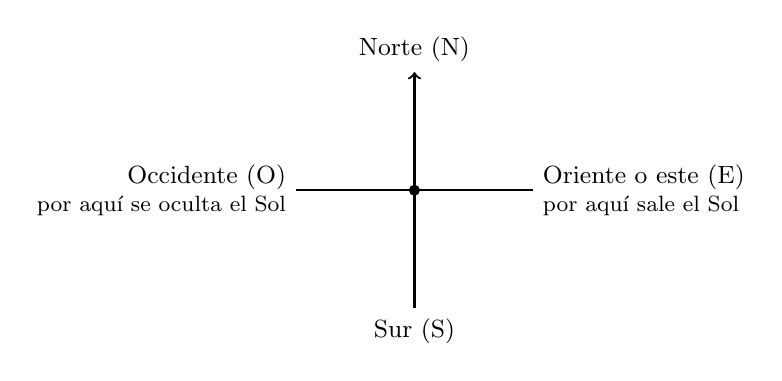
\begin{tikzpicture}[font=\small]
  \draw[->, thick] (0,0) -- (0,1.5) node[above] {Norte (N)};
  \draw[thick] (0,0) -- (0,-1.5) node[below] {Sur (S)};
  \draw[thick] (0,0) -- (1.5,0) node[right, align=left] {Oriente o este (E)\\[-1pt]
    {\footnotesize por aquí sale el Sol}};
  \draw[thick] (0,0) -- (-1.5,0) node[left, align=right] {Occidente (O)\\[-1pt]
    {\footnotesize por aquí se oculta el Sol}};
  \fill (0,0) circle (2pt);
\end{tikzpicture}
\end{center}

\begin{nota}
\textbf{Antes de la clase}, confirma por qué pared del salón entra el Sol a primera hora: esa
es el oriente, y así la práctica oral usa direcciones reales y no inventadas. Un dato de Cali
que ayuda: los Farallones, la cordillera que se ve desde toda la ciudad, quedan al occidente,
así que por la tarde el Sol se oculta detrás de ellos. Si el día está nublado, usa esa
referencia.
\end{nota}

\begin{center}
{\renewcommand{\arraystretch}{1.3}
\begin{tabularx}{\linewidth}{@{}l l X@{}}
  \toprule
  \textbf{Momento} & \textbf{Min} & \textbf{Actividad}\\
  \midrule
  Tarea 1 & 0--8 & Recoger la Tarea 1. Revisar en voz alta solo la pregunta 3c (Mariana
    «en la Calle 2 con Carrera 1»): recuerda que el orden y el punto de partida son parte del
    acuerdo. Las respuestas completas están en los bloques de solución de \texttt{semana-03/tarea.tex}.\\
  Enganche & 8--15 & Pregunta al grupo: «a las 6:55, ¿por qué ventana entra el Sol?». Si el
    día está despejado, que alguien lo señale. «Tatiana llega a Cali y le dicen: \emph{el
    hotel queda al norte del parque}. ¿Cómo sabe hacia dónde es el norte si no conoce la
    ciudad?»\\
  Explicación & 15--27 & Con la rosa de los vientos en el tablero (figura de arriba): el Sol sale
    por el \textbf{oriente} y se oculta por el \textbf{occidente}; parados mirando hacia el
    oriente, el \textbf{norte} queda a la izquierda y el \textbf{sur} a la derecha. Por
    costumbre, los mapas se dibujan con el norte arriba; por eso en un mapa el oriente queda a
    la derecha y el occidente a la izquierda. Escribir las abreviaturas N, S, E (\emph{este},
    otro nombre del oriente) y O. Dibujar el plano del colegio de la guía y leerlo con el
    grupo: ¿qué queda al sur del patio? (el coliseo), ¿y al oriente? (la cafetería). Las
    preguntas del norte y el occidente se dejan para el taller.\\
  Práctica oral & 27--30 & Todos de pie, mirando hacia el oriente del salón: «señalen el
    norte», «den media vuelta: ¿hacia dónde miran ahora?», «¿qué queda a su espalda?».\\
  Taller 1 & 30--52 & En parejas, cada uno entrega su hoja. Pregunta 1: repaso de la
    cuadrícula (fila, columna); preguntas 2 y 3: puntos cardinales en el plano del colegio y
    en el mapa del barrio. Circular por los puestos con las preguntas de la nota de abajo.\\
  Cierre & 52--55 & Idea clave: \emph{los puntos cardinales no dependen de quién mire; un mapa
    con el norte arriba lo entiende cualquiera}. Anunciar que la próxima semana los cambiaremos
    por números: el plano cartesiano.\\
  \bottomrule
\end{tabularx}}
\end{center}

\begin{nota}
Errores frecuentes para vigilar durante el taller:
\begin{itemize}
  \item Confundir izquierda con occidente \emph{fuera del mapa}: «a la izquierda» depende de
        hacia dónde mira la persona; «al occidente» no. La pregunta 2c del taller está hecha
        para eso: mirando al oriente, la izquierda es el norte.
  \item Describir con una sola dirección un lugar que exige dos («la biblioteca está al
        norte del museo»): pide contar las cuadras en cada dirección por separado.
  \item No uses todavía pares $(x, y)$ ni números en los ejes del mapa: el plano cartesiano
        llega en la sesión 004. En el taller el mapa del barrio va sin números a propósito;
        los estudiantes cuentan cuadras.
\end{itemize}
\end{nota}

\textbf{Respuestas del taller.} Están en \texttt{taller-clave.pdf}. En resumen: 1) Juliana; la
posición correcta de Andrés es $(B, 4)$. 2) Biblioteca; portería; biblioteca y portería.
3) a) 2 cuadras al oriente y 2 al norte; b) 4 al occidente y 3 al norte; c) 3 al occidente,
en la misma calle.

\end{document}
